\section{Native Language Identification}
\label{sec:nli}

NLI is usually the first step in any second language error correction or author
profiling system. Identifying the native language of an anonymous text was first
popularized by Koppel et al. (2005). Brooke and Hirst (2012) do an extensive
survey of NLI feature efficacy, and develops a robust model that works well when
used across corpora. NLI tasks are most commonly evaluated solely on a small
learner corpus usually consisting of student essays (as shown in
section~\ref{sec:datasets}). It was previously thought that lexical features
would be biased or overfit towards essay topics, but a cross-corpus evaluation
showed that this was not the case~\cite{2012-robust-nli}.

For a more in-depth discussion of authorship attribution, we recommend the
reader consult two well-known surveys~\cite{aa-survey}~\cite{koppel-survey}.
Many techniques common to authorship attribution and author profiling are also
relevant to NLI.

As mentioned in section~\ref{sec:datasets}, the ICLE was an early popular
dataset to evaluate NLI tasks, especially using a subset of five European
languages partitioned by Koppel et al. (2005). A table has been created
(Table~\ref{table:nli-comp}) to portray the summary described in Brooke and
Hirst (2012). In addition to the results displayed in the table, Wong and Dras
also attempted to perform dimensionality reduction with LDA~\cite{lda} as
feature generation; however, this was not a successful method.

Techniques for NLI can be categorized into two methods: feature-based and
likelihood-based. Feature-based methods rely on informative features derived
from the text and are fed to standard machine learning algorithms (usually SVM
or MaxEnt). Likelihood-based methods learn a probabilistic model (usually a
grammar or language model) for each L1 and assign a label based on the maximum
likelihood model. We now move onto specific techniques applied in NLI.

\subsection{Techniques in Native Language Identification}
\label{subsec:nli}

The first feature-based method~\cite{tsur} found that incredibly simple
top two hundred frequent bigram character features fed to SVM led to $66\%$
accuracy on the five native languages. They claimed that word choice of
non-native speakers is influenced by the phonology of their native language (as
evidenced by the effectiveness of the character features). This approach is
compared to a unigram words baseline which achieved only $47\%$ accuracy. They
finally hypothesized that using a spoken-language corpus would achieve even
stronger results favoring character bigrams. Their reasoning was that much less
conscious effort is put into speaking than writing. For analyzing transcripts of
spoken words, the ICNALE corpus may be applicable, described in section 3.

NLI has also been approached through contrastive
analysis~\cite{wong2009contrastive}: the idea that errors in text are influenced
by the native language of the author. They investigated three error types as
features: subject-verb disagreement, noun-number disagreement, and determiner
misuse. These error types are then used as ``stylistic markers'' for NLI
features with an SVM classifier. To find these errors in text, they used an open
source grammar
checker\footnote{\url{http://queequeg.sourceforge.net/index-e.html}}, as opposed
to professionally edited text. Interestingly, ANOVA showed that the features had
a measurable effect, but after combining their contrastive features with
existing methods, they were not able to significantly increase the
classification accuracy from Koppel et al. (2005).

The previous authors~\cite{wong-rules} follow their work on contrastive
analysis, attempting to amend its shortcomings. Instead of error types, they use
two different features obtained from grammatical parse trees: horizontal slices
(production rules) and parse rerankings. They claim these are the first pure
syntactic features used in NLI\@. For the production rules, they immediately
applied information gain dimensionality reduction. The reranking features are
those contained in the Charniak parser\footnote{\url{http://cs.brown.edu/~ec/}}
and Stanford
Parser\footnote{\url{http://nlp.stanford.edu/software/lex-parser.shtml}} trained
on the Wall Street Journal. Unlike the previous two attempts, the authors found
MaxEnt to outperform SVM as the classifier. Additionally, five-fold cross
validation was performed (as opposed to ten-fold), which means the accuracies
cannot be precisely compared with previous work. In any event, they report a
final accuracy of $80\%$, which was the highest reported as of 2012.

\begin{table}[t]
  \begin{center}
    \begin{tabular}{llr}
        \hline
        \hline
        \textbf{Paper} & \textbf{Method} & \textbf{Accuracy} \\
        \hline
        (Tsur and Rappoport 2007) & character $n$-grams$^*$ & 66\% \\
        (Wong and Dras 2009) & syntactic errors$^*$ & 74\% \\
        (Wong and Dras 2011) & syntactic rules$^*$ & 80\% \\
        (Wong et al. 2012) & adaptor grammars$^{*+}$ & 76\% \\
        (Swanson and Charniak 2012) & tree substitution grammars$^{*+}$ & 78\%\\
        (Stolerman et al. 2013) & language family$^*$ & 80\%
        \\
        \hline
        \hline
    \end{tabular}
  \end{center}
    % can't have citations in captions for some reason...
    \caption{Summary of native language identification results listed in (Brooke
    and Hirst 2012) for the ICLE corpus; accuracies added to chart. $^*$
indicates feature-based methods and $^+$ indicates likelihood-based methods.}
    \label{table:nli-comp}
\end{table}

Wong, Dras, and Johnson (2012) explore the last author's---Mark Johnson's---adaptor
grammars~\cite{adaptor-grammars} to generate features. Simply, adaptor
grammars are a non-parametric extension to PCFGs (probabilistic context free
grammars). They can learn arbitrary-length word sequences (collocations); for
example, \emph{gradient descent} and \emph{cost function} were learned as
phrases in a machine learning topic. These adaptor grammars are used in two
ways: in the first, collocations are used as features in a MaxEnt classifier. In
the second, the grammar is trained on each class (representing native language).
At test time, the most probable grammar to have generated the text is selected.
For both tasks, the authors use five-fold cross validation on seven native
languages. In the feature-based classification, they achieved $76\%$; in the
language model-based classification, they achieved only $50\%$, a performance
similar to the unigram word baseline from Tsur and Rappoport (2007).

Swanson and Charniak (2012) made use of tree substitution grammars (TSGs)~\cite{tsgs}. TSGs are a tree-rewriting formalism that defines operations on
partial (parse) tree objects. For example, subtrees may be added or removed from
a base tree. Benefits of using this method are priors which prefer smaller
production rules and the ability to capture long-range dependencies. Various
induction methods are compared to generate features, and five-fold cross
validation on seven native languages is performed. All TSG features outperformed
the CFG baseline (at $73\%$). The highest TSG induction method was Bayesian
induction at $78\%$.

Massung, Zhai, and Hockenmaier (2013) also make use of grammatical parse tree features, but mainly
focus on their structural aspects as opposed to the syntactic category labels.
In one classification task, they found these features to work well in
determining the nationality of student essay writers from the CEEAUS dataset.
These structural parse tree features may be applicable in other tree-based
objects such as adaptor grammars, tree substitution grammars, and dependency
parses, but this has yet to be explored.

Lastly, Stolerman, Caliskan, and Greenstadt (2013) use language family as a feature for NLI\@. Specifically,
they took ICLEv2 documents classified with low confidence using unigram features
and reclassified them into one of the Germanic, Slavic, or Romance language
families. From there, the document was classified as an L1 using a subset of
training data only from the language family it was classified as. This method is
a type of hierarchical classification problem, and achieved about a $6\%$
increase over the baseline in NLI accuracy when using information gain feature
selection.

In summary, Table~\ref{table:nli-comp} lists the comparable accuracies from
experiments run on the ICLE/ICLEv2 subset of five European languages. In general
though, accuracies between 70\% to 80\% are standard for a wide variety of
techniques and corpora.

\subsection{Shared Task in Native Language Identification}
\label{subsec:nli-shared}

The 8th Building Educational Applications workshop held a shared task dedicated
to NLI~\cite{nli-shared}. Its goal was to increase visibility of
the problem and standardize results on a larger dataset: ETS\@. In total,
twenty-nine teams participated in the shared task.

There were three separate subtasks, differentiated by what data was allowed for
training:

\begin{itemize}
    \item \textbf{Closed Training}: use only the ETS corpus for training. All
        twenty-nine teams attempted this task.
    \item \textbf{Open Training I}: use any data \emph{except} the ETS corpus
        for training; the evaluation is still done on the ETS test set. Only
        three teams attempted this task.
    \item \textbf{Open Training II}: Use any data \emph{including} the ETS
        corpus. Only four teams attempted this task.
\end{itemize}

Overall results for the closed training were relatively close; the top thirteen
teams had between $80-83.6\%$ accuracy. The open training I subtask teams
performed much lower (probably as expected) at around 33, 38, and 57$\%$
accuracy. Finally, in the open training II subtask, none of the four teams were
able to beat the highest closed score. The most useful results for evaluating
models are probably those of the closed task, since all training data is
uniform, though it is interesting to see approaches employed to increase the
amount of training data. For example, in the open subtasks, other NLI datasets
were used such as ICLE, FCE, and ICNALE (all described in
section~\ref{sec:datasets}). Additionally, some teams crawled Lang-8, also
described in section 2.

\begin{figure}[t]
\begin{center}
\begin{minipage}[c]{.45\textwidth}
    \begin{center}
    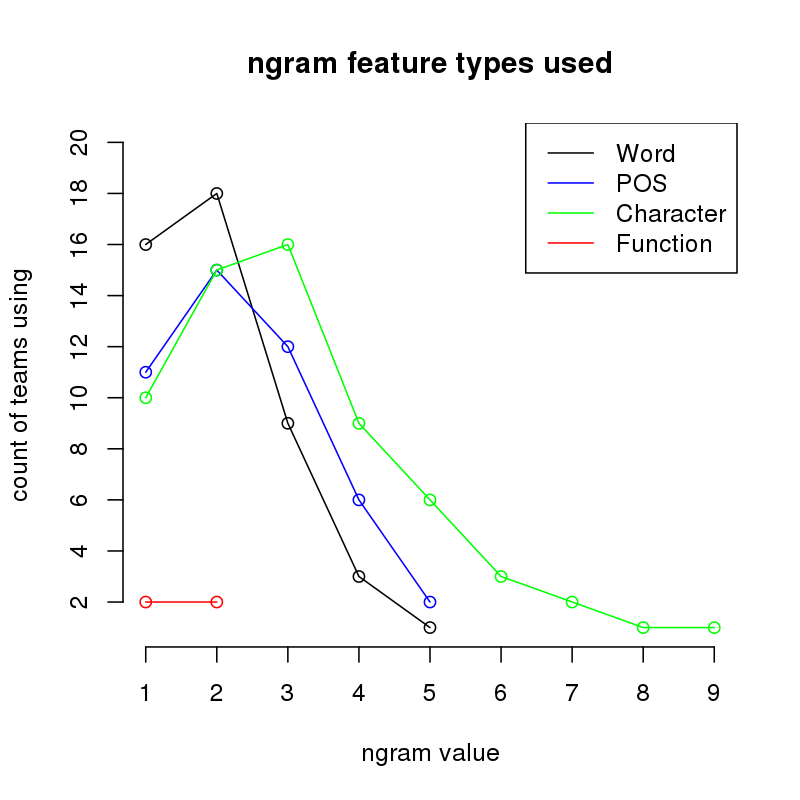
\includegraphics[width=2.3in]{ngram-comp}
    \end{center}
\end{minipage}
\hfill
\begin{minipage}[c]{.45\textwidth}
    \begin{center}
    \begin{tabular}{ll}
    \hline
    \hline
    \textbf{Classifier} & \textbf{Count} \\
    \hline
    SVM & 13 \\
    Ensemble & 4 \\
    MaxEnt & 3 \\
    DFA & 1 \\
    String kernel & 1 \\
    PPM & 1 \\
    $k$-NN & 1 \\
    \hline
    \hline
    \end{tabular}
    \end{center}
\end{minipage}
\caption{Number of teams using particular $n$-gram features (left) and number of
teams using a particular machine learning algorithm (right). DFA and PPM refer
to discriminant function analysis and prediction by partial matching.}
\label{fig:ngram-comp}
\end{center}
\end{figure}


The most common features used were $n$-grams of lexical tokens such as words or
part-of-speech tags; Figure~\ref{fig:ngram-comp} compares the $n$-grams used by
all teams. Aside from these, some less common features were grammatical:
dependency parses, TSGs~\cite{tsgs}, parse tree rules, and adaptor grammars~\cite{adaptor-grammars} were used. Spelling error features were also
captured by three of the teams. These features are all described in work in
section~\ref{subsec:nli}. Below, we outline a few of the more unique feature
representations.

Skipgrams~\cite{skipgrams} were an $n$-gram variant feature used by several
teams. Instead of considering an $n$-gram to consist of $n$ adjacent words in
the text, a $k$-skip $n$-gram allows up to $k$ words total to be skipped in a
sequence of tokens. Given the sentence ``\emph{They all studied statistics
Monday evening}'', normal 3-grams would be $\{$\emph{They all studied, all
studied statistics, studied statistics Monday, statistics Monday evening}$\}$. A
few possible 2-skip 3-grams are $\{$\emph{They all studied, They studied
statistics, They statistics Monday}$\}$. This attempts to capture important
phrases without regard to interspersed function words. Using skipgrams was shown
to reduce perplexity on a testing set, as well as offer a viable alternative to
increasing the corpus size (which is usually not feasible). Since most NLI
datasets we have examined are relatively small, using skipgrams could help
improve language modeling. While interesting, none of the teams in the top third
used skipgrams in their systems.

For one feature type, the system by LIMSI used a form of machine translation
called ``back translations''~\cite{nli-mt}. A back translation attempts to
capture a writer's lexical preference for a word sense. For example, LIMSI found
that the English word sense for \emph{awkward} is more likely to be written as
\emph{clumsy} by native Spanish speakers. These word preferences were used as
features in addition to other features: word $n$-grams, spelling mistakes, and
grammatical mistakes. Adding the back translation features slightly increased
the task's overall classification accuracy, but the team still performed poorly
overall.

The CMU-Haifa team used a ratio of passive to active verbs in their
system~\cite{nli-passives}. They operated under the common assumption that
English uses passive voice more frequently than other languages, and the amount
of passive use may vary based on the writer's L1. Recall that passive voice is a
literary technique that shifts attention away from the one performing an action.
``\emph{The passive voice is often used}'' is a sentence in the passive voice;
``\emph{English speakers often use the passive voice}'' is a sentence in the
active voice. The passive voice is characterized by the verb \emph{to be} and
the past participle of the verb. In the previous sentences, we have \emph{is
used} and \emph{use} conjugated differently. Using the passive ratio feature
exclusively yielded a $12\%$ accuracy on a $9\%$ baseline. In combination with
four other main features, the accuracy was not significantly improved. However,
further investigation could be warranted to examine the usefulness of such
stylistic composition features.

SVM was by far the most prevalent classifier employed by the teams, as displayed
in Figure~\ref{fig:ngram-comp}. Below, we outline some of the more uncommon
classifiers.

Discriminant function analysis (DFA) from statistics was used
for increased interpretability over other methods~\cite{nli-dfa}. Using this model, they were
able to find correlations between different L1s. For instance, Japanese and
Korean L1s were highly correlated in their underuse of the words $\{$\emph{all,
any, but, different, or, person, this, your}$\}$. Unsurprisingly, languages of
similar origin were also correlated---the Romance languages were often
misclassified as one another due to increased correlation of $n$-gram tokens.
Unfortunately, this team performed poorly overall.

Originally designed to operate on DNA sequences, the string kernel model~\cite{2013-stringkernel} is given a stream of characters. Specifically,
a kernel based on local rank distance is used for native language
identification. The simplest string kernel function $f(w_1,w_2)$ counts the
number of substrings of a particular length that $w_1$ and $w_2$ share. It is
also quite intuitive to introduce a normalized version that is not biased by
long words. Local rank distance is then an extension that counts the sets of
\emph{similar} $n$-grams between $w_1,w_2$. In their NLI context, each word was
actually a character $n$-gram. This method has the advantage that no syntactic
information is needed; no parsing or even sentence or word segmentation is
required. In training, they found that $n\in[5,8]$ gave the best results,
allowing them to take third place overall in the closed task.

Similar to the string kernels previously, Bobicev (2013) uses a method which
requires very little text processing: prediction by partial matching (PPM), a
statistical compression method. The output of PPM is a language model which can
be used to find the highest likelihood L1 given some unknown text. Both words
and characters were used as tokens, though character features performed much
worse than words, obtaining a precision of $37\%$ (compared to $70\%$ from the
word tokens) on the 9,900-document training set. This performance placed the PPM
features in the bottom third of contestants.

\begin{table}[t]
\begin{center}
    \begin{tabular}{llr}
        \hline
        \hline
        \textbf{Paper} & \textbf{Method} & \textbf{Accuracy} \\
        \hline
        \hline
        (Jarvis et al. 2013) & SVM on lexemes, lemmas, POS & 83.6\% \\
        \hline
        (Bykh and Meurers 2014) & ensemble many lexical/syntactic & 84.8\% \\
        \hline
        (Ionescu et al. 2014) & character string kernels & 85.3\% \\
        \hline
        \hline
    \end{tabular}
    \caption{Increasing state-of-the-art NLI accuracy results for the ETS
    dataset.}
    \label{table:ets}
\end{center}
\end{table}

In conclusion, most methods used by teams in the NLI shared tasks were very
standard (\emph{e.g.} $n$-grams of words with SVM). In fact, the winning
team~\cite{jarvis} with 83.6\% accuracy used SVM with unigram to trigrams of
log-entropy weighted lexemes, lemmas, and POS tags. A small number of teams
investigated some unique text representations and classification techniques.
Given options between feature-based and likelihood-based strategies, most teams
focused on features. While not always successful, these new methods can be
further explored and analyzed in future work. Table~\ref{table:ets} summarizes
the results discussed on the ETS dataset. After the contest ended, others
have surpassed the highest-scoring Jarvis et al.\ team.

First, Bykh and Meurers (2014) considered an ensemble of various
features, consisting of context-free grammar rules and forty $n$-gram
representations of words, POS tags, and lemmas for $n\in[1,10]$. They found
training a separate classifier for each feature type gave definite advantages
over concatenating feature vectors.

Second, Ionescu, Popescu, and Cahill (2014) improved over Bykh and Meurers
(2014) by using only
character-based features. However, the way that the character features are used
is advanced. They combined various string kernels with two learning methods,
kernel ridge regression and kernel discriminant analysis. We suggest that the
reader consult their paper for a more in-depth description of these tools. Their
best results were when string lengths were in the range $[5,8]$. Seven of their
kernel and learning combinations outperformed the first place shared task
team~\cite{jarvis}, and their best two combinations best the Bykh and Meurers
score. Their highest-scoring setup was kernel discriminant analysis on a
weighted combination of a presence bits kernel (dot product of occurring
characters) and the intersection string kernel.
